\section{SRNG-disjoint path problem}
\subsection{Shared Risk Node group}
\revtao{
The concept of SRLG can also be extended to encompass the shared risk node group (SRNG) where instead of links, nodes belong to certain risk groups, as shown in Fig.\ref{fig:SRNG}(a). Though we only illustrate the case when a node belongs to a risk group, there is no limit to the number of risk groups that a node could belong to multiple SRNGs. When nodes represent routers in a communication network, all routers of the same manufacturer would belong to a risk group since a bug affecting the router model would affect them all.}

\revtao{Shared-Risk Link Groups (SRLG’s) and Shared Risk Node Groups (SRNG’s) are becoming critical in survivable optical network design. In Sec.\ref{sec:Trap problem and solution overview }, we have proposed a algorithm to solve SRLG-disjoint path problem. In this subsection, we talk about the extention of our algorithm so that solve the shared risk node group(SRNG) disjoint path problem.}


\subsection{Problem description}
A shared risk node group (SRNG) is a group of nodes that share a component whose failure causes the failure of all nodes in the group. A node can belong to multiple SRNGs.

Similarly as SRLG problem's definition, let $\mathbb{R}$ be the risk (failure) set in the network. For $r_i \in \mathbb{R}$, its SRNG is the node set associated with risk $r_i$, denoted as $\mathbb{R}_{r_i}$, where $1\leq i\leq \chi$ and $\chi=|{\mathbb{R}}|$ is the number of risks/SRNGs.  In Fig.\ref{fig:SRNG}(a), the network includes three SRNGs $\mathbb{R}_{r_1}=\{v_1,v_4\}$, $\mathbb{R}_{r_2}=\{v_2,v_3\}$, $\mathbb{R}_{r_3}=\{v_3,v_5\}$. In this example, node $v_3$ is in two SRNGs $\mathbb{R}_{r_2}$ and $\mathbb{R}_{r_3}$.


Let $r_P$ denote the risk set that impacts a path $P$, that is $r_P=\{r\in \mathbb{R}$: path $P$ contains nodes in $\mathbb{R}_r\}$. In Fig.\ref{fig:SRNG}(a), the node set on the AP is $\mathbb{AP}=\{s,v_1,v_2,d\}$ with $v_1\in \mathbb{R}_{r_1}$, $v_2\in \mathbb{R}_{r_2}$, the risk set of AP is ${r}_{{AP}}=\{r_1, r_2\}$.

SRNG-disjoint paths share no common risks among themselves, that is, the failure of a path due to a risk would not affect other paths. Fig.\ref{fig:SRNG}(c) shows two SRNG-disjoint paths, denoted as AP and BP. As these two paths share no common risk, if AP fails, BP can still work. This paper focuses on finding  two SRNG-disjoint paths for path protection, which can be described as follows.


\textbf{Min-Min SRNG-disjoint routing problem.} Given a graph $G(\mathbb{V},\mathbb{E})$, a weight $w_{e_i}$ associated with each link $e_i\in \mathbb{E}$, a source  $s$ and a destination  $d$,  find a pair of SRNG disjoint paths from $s$ to $d$ (denoted as $AP$ and $BP$), thus that  the smallest path weight of the two disjoint paths is minimized, that is,

\begin{equation}
\begin{array}{*{20}{c}}
   {\mathop {minimize}\limits_{AP,BP} } & {\min \left( {{w_{AP}},{w_{BP}}} \right)}  \\
   {subject\ to} & {{r_{AP}} \cap {r_{BP}}{\rm{ = }}\phi }  \\
   {} & {\mathbb{AP} \cap \mathbb{BP}{\rm{ = }}\phi }  \\
\end{array}
\label{eq:problem definition}
\end{equation}
where ${w_{AP}}$ and ${w_{BP}}$ are the path weights of AP and BP, respectively, $\mathbb{AP}$ and $\mathbb{BP}$ are the node sets on paths AP and BP, respectively, ${r_{AP}}$ and ${r_{BP}}$ are the risk sets that impacts AP and BP, respectively.


\subsection{SRNG transform to SRLG method}

\revtao{
In this subsection we discuss shared-risk node groups. We supposed a transformation technique as shown in Fig.\ref{fig:SRNG} for finding out two SRNG-disjoint paths in scenarios where more than one node shares a common risk of failure. We identify such scenarios where more than one node shares a common risk of failure as shared risk node groups (SRNG’s).
We assume that each node can be part of not only one SRNG and we also assume that the size of each SRNG is not limited to two adjacent nodes sharing an edge between them as shown in Fig.\ref{fig:SRNG}.(a) node $v_3$.
The SRNG transform to SRLG method is polynomial-time approach. Each node $v_n$ is split into two nodes $v_{n_{in}}$ and $v_{n_{out}}$ that are connected by a link with zero weight.
}



\begin{figure}[tp]
  \centering
  % Requires \usepackage{graphicx}
  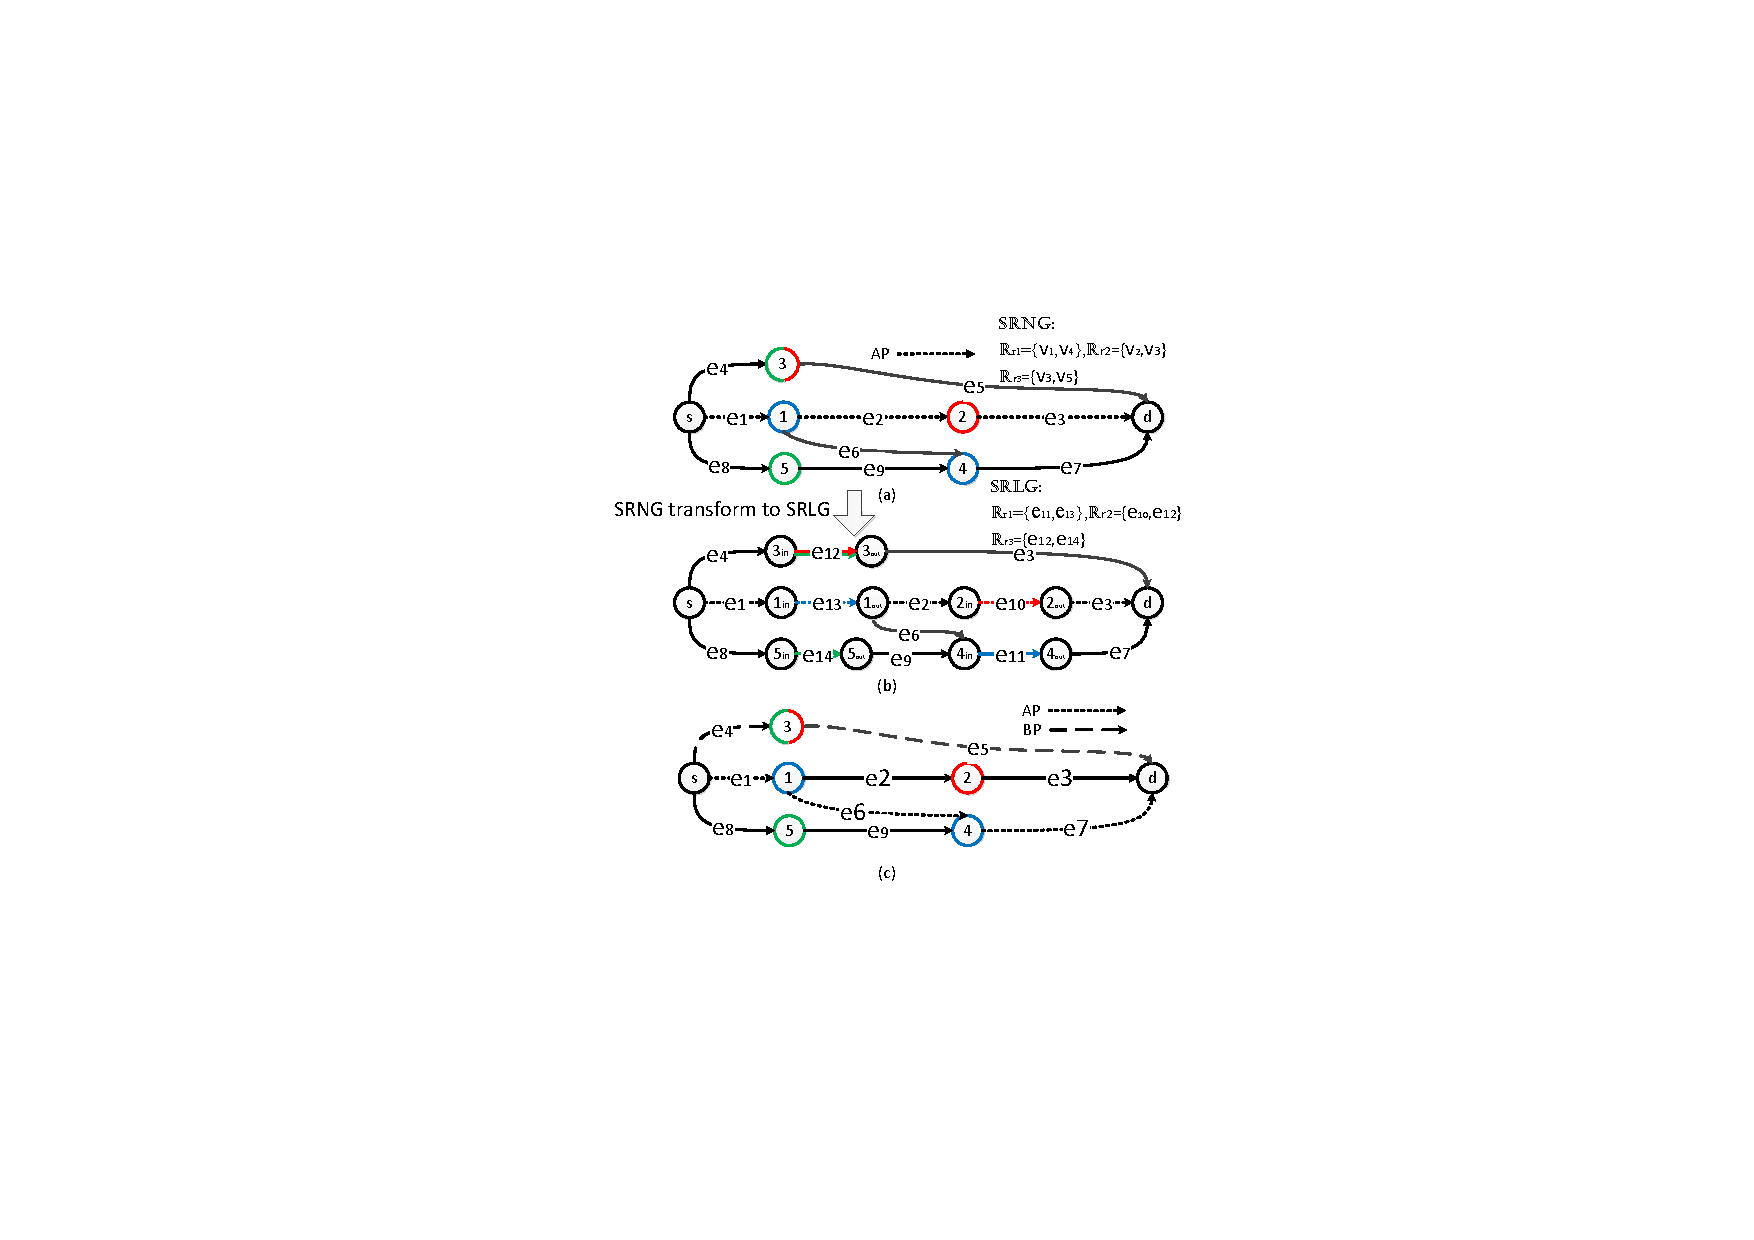
\includegraphics[width=3.0in]{franz/SRNG}
  \caption{(a) A graph with five SRLGs: $\mathbb{R}_{r_1}=\{v_1,v_4\}$,$\mathbb{R}_{r_2}=\{v_2,v_3\}$,$\mathbb{R}_{r_3}=\{v_3,v_5\}$. (b) SRNG transform to SRLG. $\mathbb{R}_{r_1}=\{v_1,v_4\}\rightarrow \{e_{13},e_{11}\}$,$\mathbb{R}_{r_2}=\{v_2,v_3\}\rightarrow \{e_{10},e_{12}\}$,$\mathbb{R}_{r_3}=\{v_3,v_5\}\rightarrow \{e_{12},e_{14}\}$. (c) AP and BP in the graph.}\label{fig:SRNG}
  \label{fig:SRNG}
\end{figure}
%\begin{figure}[tp]
%  \centering
%  % Requires \usepackage{graphicx}
%  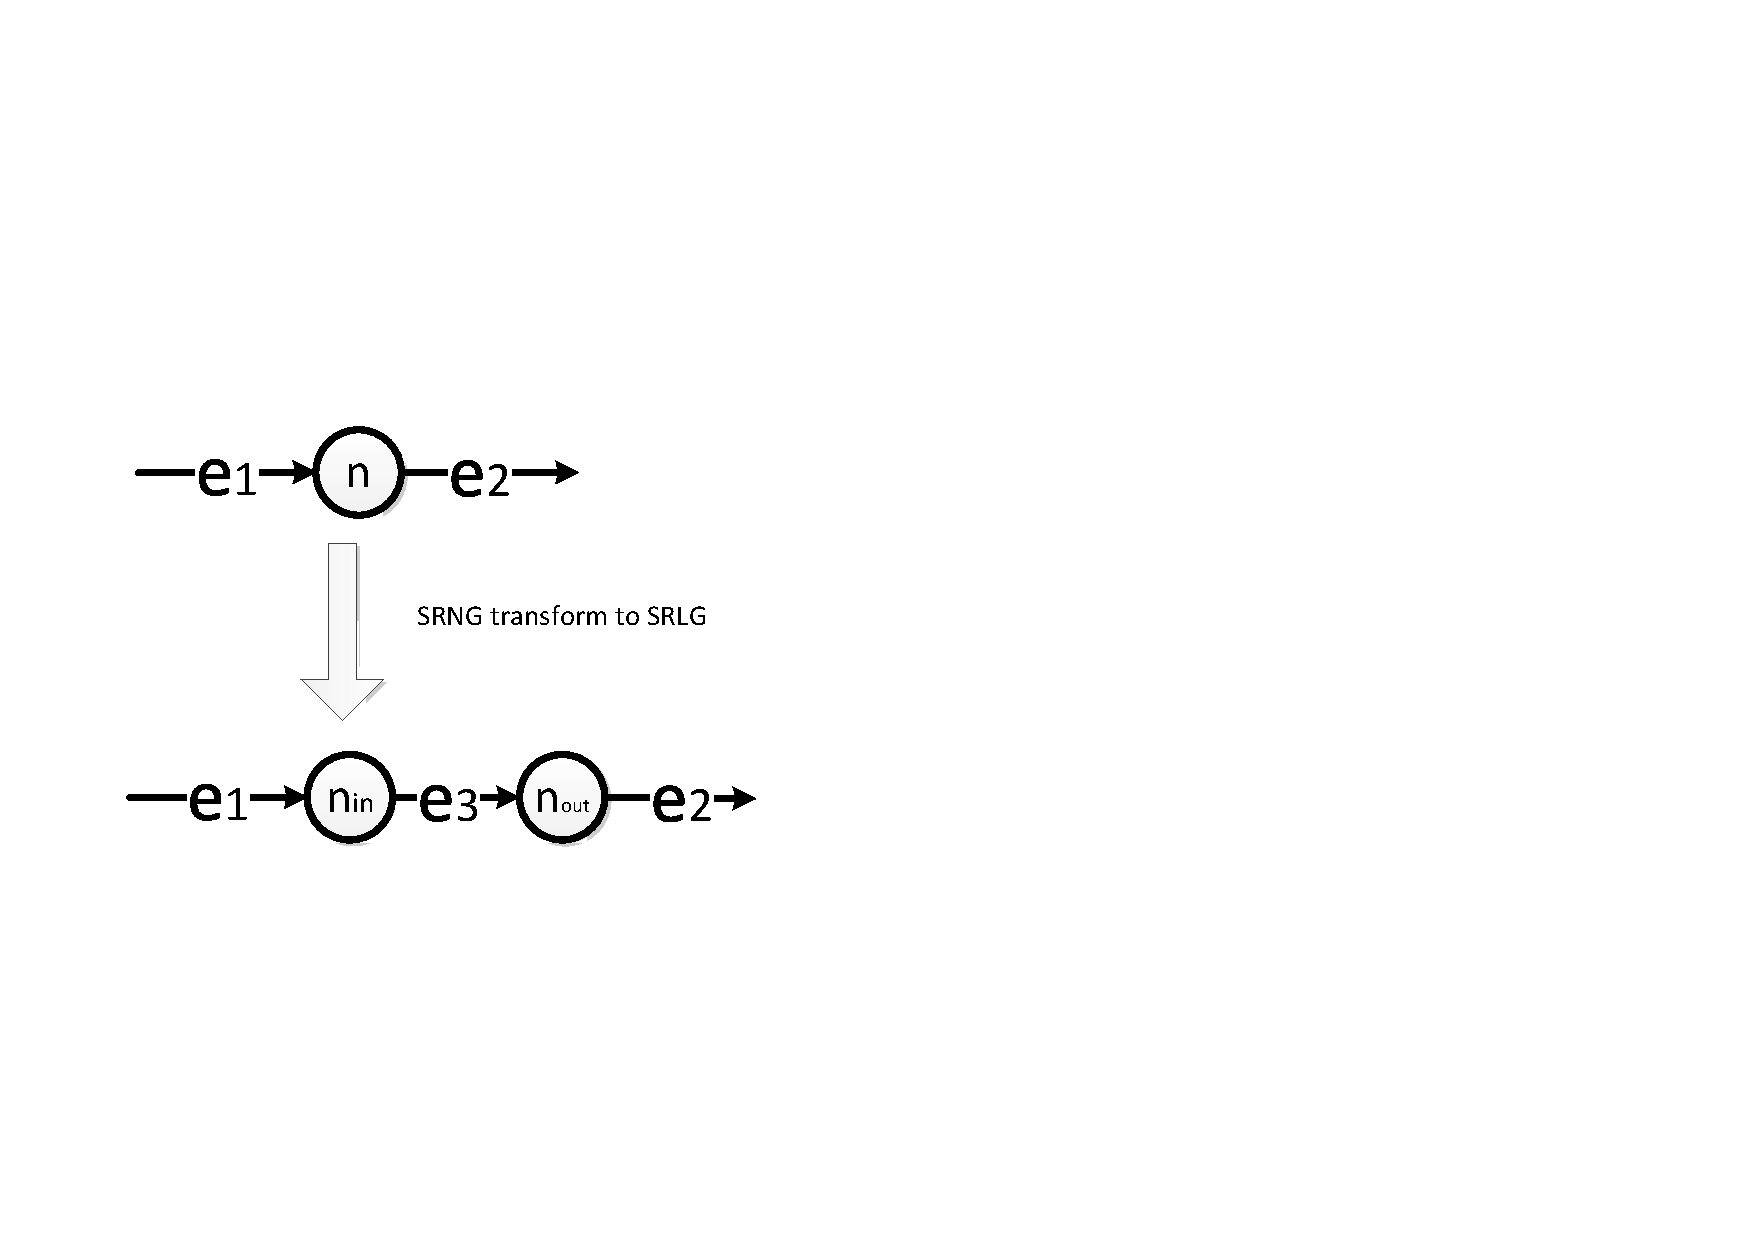
\includegraphics[width=2.0in]{franz/node2edge}
%  \caption{SRNG transform to SRLG. $\mathbb{R}_{r}=\{v_n,\ldots\}\rightarrow \{e_{3},\ldots\}$}\label{fig:node2edge}
%  \label{fig:node2edge}
%\end{figure}


\subsection{DOMAIN-DISJOINT PATHS}
\revtao{The domain-disjoint paths problem is formally defined as follows:}
